\documentclass{article}
\usepackage{enumerate}
\usepackage{amsfonts, amscd, amsmath, amssymb}
\usepackage{graphicx}

\oddsidemargin -0.3cm
\evensidemargin 0cm
\textwidth 16.5cm
\textheight 21cm

\def\N{\mathbb N}
\def\Z{\mathbb Z}
\def\Q{\mathbb Q}
\def\R{\mathbb R}
\def\C{\mathbb C}

\title{Tema 1. Introducci\'o}
\date{}

\begin{document}
\maketitle


\tableofcontents

\section{Senyals i Sistemes}

El terme {\it senyal} fa refer\`encia a qualsevol informaci\'o mesurable 
generada per un fen\`omen f\' \i sic. Alguns exemples de senyals s\'on:

\begin{itemize}
\item la veu humana, o millor dit, la mesura de la veu humana, \'es a dir,
la variaci\'o de la presi\'o de l'aire a mida que parlam,
\item l'evoluci\'o de la intensitat el\`ectrica en un circuit el\`ectric,
\item una fotografia, o millor dit, el valor de lluminositat o color en cada
punt del paper fotogr\`afic.
\end{itemize}

En termes matem\`atics el concepte de {\it senyals} es correspon amb la 
noci\'o de funci\'o. Aquestes funcions poden \'esser uni-dimensionals 
(com en el cas de la veu o de la intensitat el\`ectrica), bi-dimensionals 
(la fotografia) o, en general, $n$-dimensionals. A m\'es a m\'es cal observar
que no tots els senyals s\'on funci\'o del temps sin\'o que tamb\'e poden
representar variacions en l'espai (com en el cas de les fotografies) o
qualsevol altre magnitud. 

\begin{figure}[htbp]
\begin{center}
\begin{tabular}{ccc}
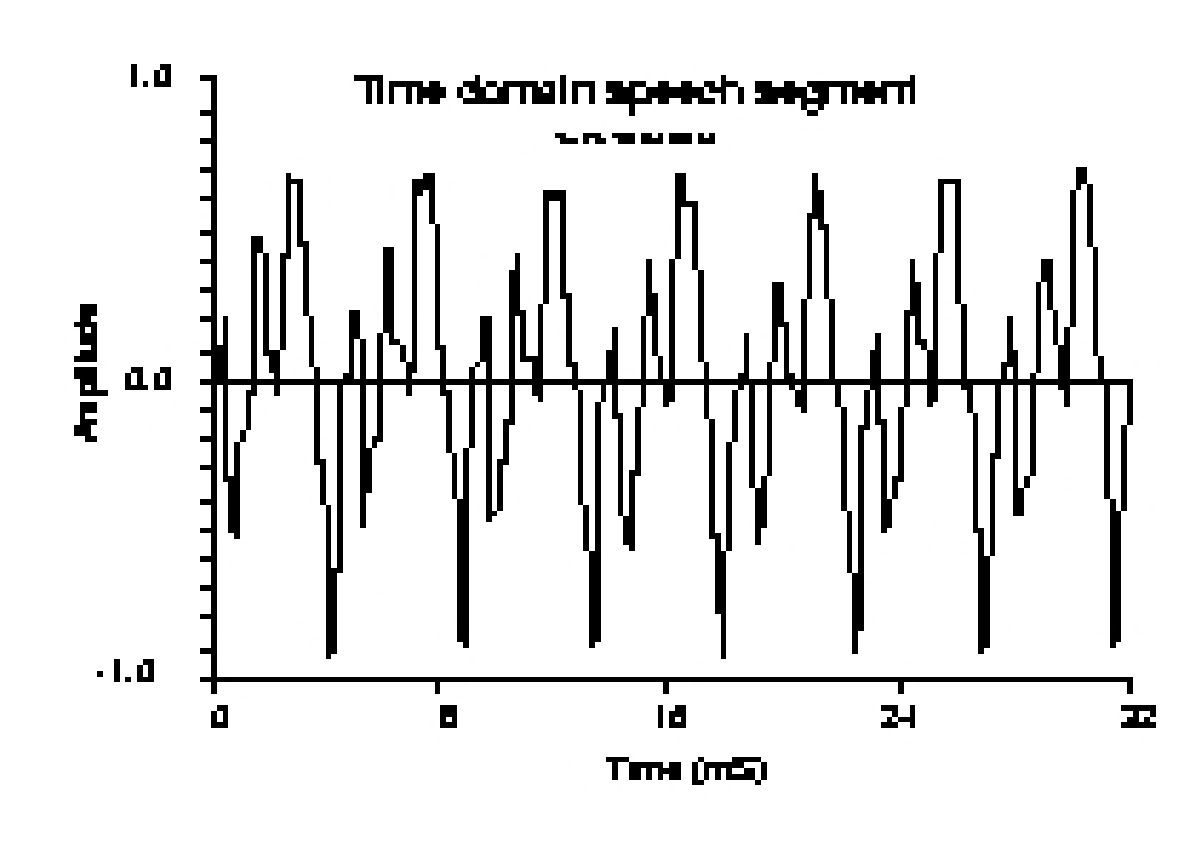
\includegraphics[width=60mm]{imatges/senyalveu.eps} & &
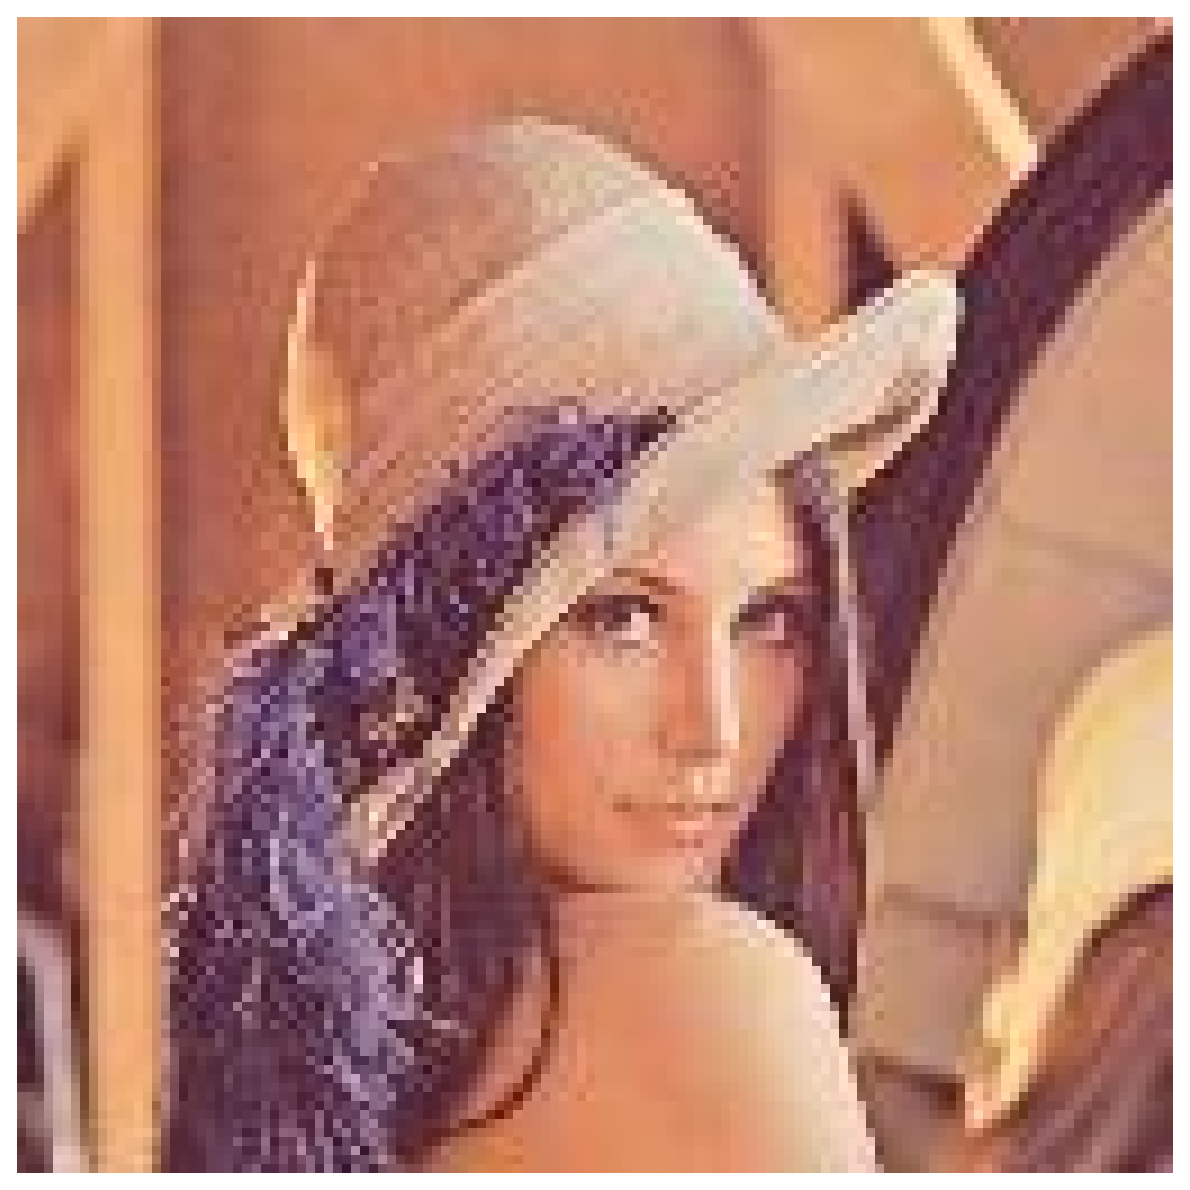
\includegraphics[width=50mm]{imatges/lena.eps}
\end{tabular}
\caption{Dos examples de senyals. A l'esquerra, un senyal de veu. A la dreta,
una imatge} 
\label{senyals.fig}
\end{center}
\end{figure}

Un {\it sistema} o {\it filtre} \'es qualsevol proc\'es que modifica un senyal
i es pot mo\-delar matem\`aticament com un operador que actua sobre 
una funci\'o
(el senyal d'entrada) per donar una nova funci\'o (el senyal de sortida).
Esquem\`aticament:

\begin{figure}[htbp]
\begin{center}
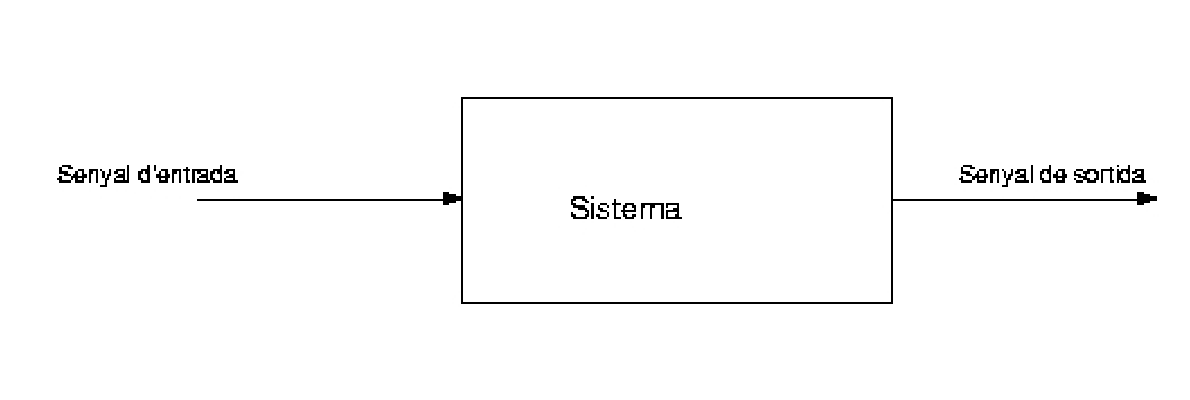
\includegraphics[width=9cm]{imatges/sistema.eps}
\caption{Representaci\'o esquem\`atica d'un sistema o filtre}
\label{sistema.fig}
\end{center}
\end{figure}

Com a exemples de sistemes tenim els seg\"uents:
\begin{itemize}
\item un circuit el\`ectric,
\item un micr\`ofon,
\item el zoom d'una c\`amara fotogr\`afica.
\end{itemize}

El segon d'aquests exemples ens permet ilustrar el fet que els senyals 
d'entrada i de sortida d'un sistema poden \'esser de natures diferents:
en el cas del micr\`ofon, l'entrada \'es una variaci\'o en la pressi\'o de 
l'aire i la sortida \'es una variaci\'o en la intensitat el\`ectrica.
En els altres dos exemples, no obstant, els senyals d'entrada i de sortida
s\'on del mateix tipus.
 

\section{An\`alisi de Fourier}
Una de les eines b\`asiques per a l'estudi dels senyals \'es l'an\`alisi
de Fourier. Recordem que l'an\`alisi de Fourier t\'e el seu or\'igen en
l'estudi, per part de Jean Baptiste Joseph Fourier (1768-1830), de la 
propagaci\'o de la calor. En 1807 Fourier va proposar la utilitzaci\'o de 
sinusoides per a la representaci\'o dels senyals obtinguts en mesurar 
variacions de temperatura. El mateix tipus d'an\`alisi es pot aplicar a 
qualsevol altre tipus de senyal.

El fet que qualsevol senyal provenent del mon f\'\i sic, per complexe que 
sigui, pugui \'esser descomposada en una suma de funcions simples (les 
sinusoides) fa de l'an\`alisi de Fourier una eina fonamental en l'estudi
dels senyals. Donat que una sinusoide es defineix per dos 
par\`ametres, la seva freq\"u\`encia i la seva amplitud, es pot interpretar 
l'an\`alisi de Fourier com un m\`etode per trobar quines s\'on les 
freq\"u\`encies que defineixen el nostre senyal, aix\'i com el p\`es o 
import\`ancia de cada una d'elles (en altres paraules, ens permet fer un
{\bf an\`alisi espectral} dels senyals).  

L'an\`alisi de Fourier tamb\'e es pot aplicar a l'estudi dels sistemes.
En el Tema 3 veurem com es classifiquen els sistemes i la seva 
caracteritzaci\'o freq\"uencial.

En el Tema 2 es fa un rep\`as dels fonaments de la Teoria de Fourier i de les
principals propietats de les transformades de Fourier.


\section{Senyals i Sistemes Discrets}
La popularitzaci\'o dels primers ordinadors digitals durant els anys 60 i 70
va proporcionar una potent eina de c\`alcul als enginyers i matem\`atics.
No obstant, per utilitzar aquestes eines va \'esser necess\`aria l'adaptaci\'o
de les dades dels problemes a un format que els ordinadors pogu\`essin
manejar. En el cas dels senyals, aix\'o implica la seva {\bf digitalitzaci\'o}.

El proc\'es de digitalitzaci\'o compr\`en dos pasos:
\begin{itemize}
\item {\bf discretitzaci\'o} de la variable de la qual depenen els valors
del senyal (temps, espai, etc.), ja que l'ordinador no pot enmagatzemar un
nombre infinit de valors.
\item {\bf quantitzaci\'o} dels valors del senyal, ja que l'ordinador
no pot enmagatzemar les dades amb una precissi\'o infinita.
\end{itemize}

L'estudi formal del problema de la discretitzaci\'o dels senyals continus
ens portar\`a introduir el concepte de {\it distribucions} i, eventualment,
al Teorema de Shannon. Aquest estudi es dur\`a a terme en el Tema 2.

En el Tema 3 s'explicar\`a com les eines de l'an\`alisi de Fourier es poden
aplicar als senyals discrets i veurem un algoritme r\`apid per al c\`alcul
del la Transformada de Fourier d'un senyal discret (la {\bf FFT}).

\section{Senyals aleatoris. Renou}
En l'estudi de la natura apareixen uns senyals pels quals no podem
predir el seu comportament en un lloc o instant determinat per\`o que
est\'an sotmesos al principi de regularitat estad\'\i stica. Aquest senyals
reben el nom de {\bf renou} i es el seu comportament es pot modelar
amb m\`etodes estad\'\i stics.

El renou, en general, es combina amb els senyals mesurats, desvirtuant les 
dades originals. Al llarg del curs veurem algunes t\`ecniques dissenyades per 
eliminar o reduir l'efecte del renou damunt dels senyals.

\section{Processament Digital del Senyal (DSP)}
El terme Processament Digital del Senyal fa refer\`encia als fonaments 
matem\`atics, els algoritmes i les t\`ecniques utilitzades per a la 
manipulaci\'o de senyals digitals. Aix\'o incluo una amplia varietat
d'objectius: millora d'imatges, reconeixement de veu, compressi\'o de dades
per a enmagatzemament/transmissi\'o, etc. El DSP \'es un bon exemple 
d'interdisciplinareitat entre diferents branques de la ci\`encia 
(Figura \ref{interdiscDSP}).
L'esquema de la Figura \ref{aplicacionsDSP}  
mostra algunes de les aplicacions del DSP.

\begin{figure}[htbp]
\begin{center}
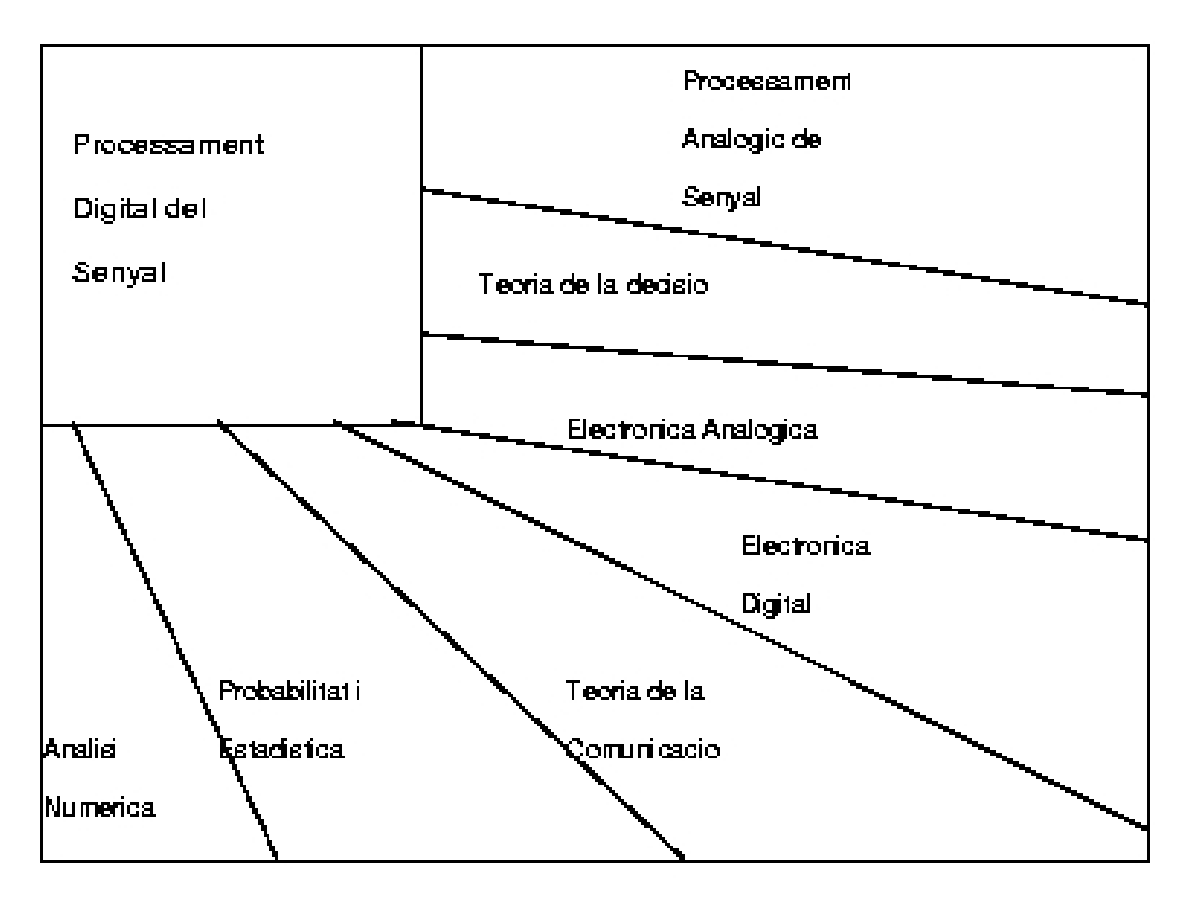
\includegraphics[width=9cm]{imatges/interdiscPDS.eps}
\caption{\cite{Schmidt}. \`Arees de la ci\`encia que intervenen en el 
desenvolupament del Processament Digital de Senyal}
\label{interdiscDSP.fig}
\end{center}
\end{figure}

\begin{figure}[htbp]
\begin{center}
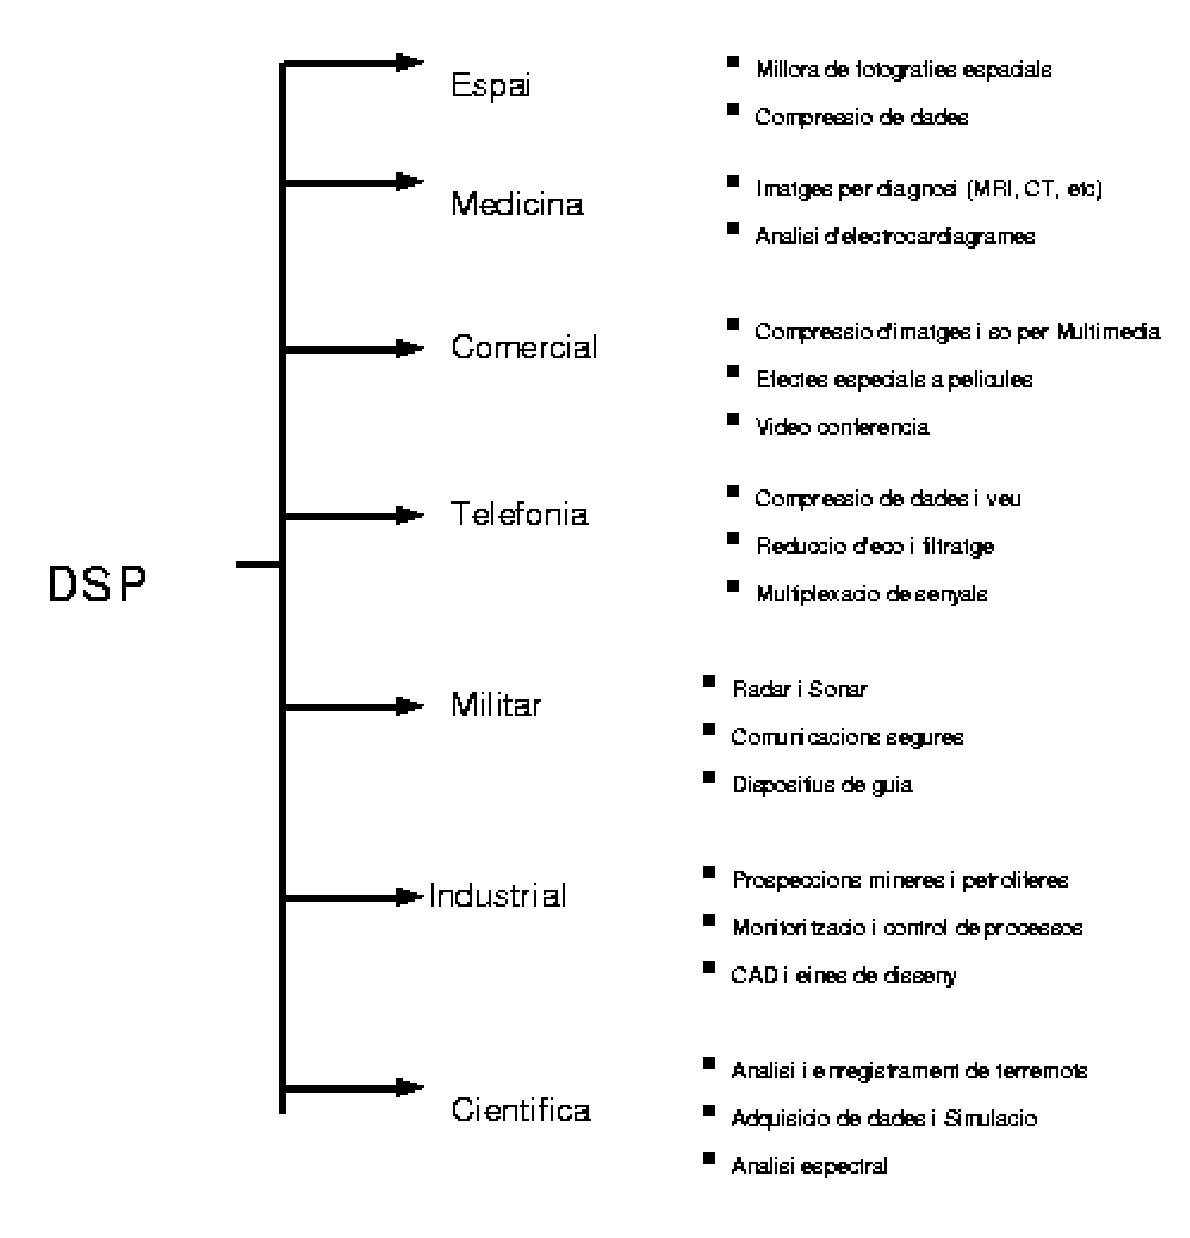
\includegraphics[width=9cm]{imatges/aplicacionsPDS.eps}
\caption{\cite{Schmidt}. Aplicacions del Processament Digital de Senyal}
\label{aplicacionsDSP.fig}
\end{center}
\end{figure}


Aquest curs intenta donar una base per als estudiants interessats en
el Processament Digital de Senyals, amb especial \`emfasi en el 
Processament d'Imatges. En els primers temes es presentaran, de forma rigorosa
per\`o no exhaustiva, les eines matem\`atiques b\`asiques per al disseny
d'algoritmes de processament de senyal i la resta de temes es dedicaran a
descriure algoritmes 'cl\`assics'. Tamb\'e es presentaran casos pr\`actics 
d'aplicaci\'o d'aquests algoritmes. 


\end{document}

